\subsection{Osnovna svojstva palindroma}

U cijelom ovom potpoglavlju duljina palindroma je
fiksna i označava se sa $m$.
Iz definicije slučajnih varijabli $\tsvar{Y}_i$ očito je da
je $\tsvar{Y}_m,\ldots,\tsvar{Y}_n$ niz $(m-1)$-zavisnih slučajnih varijabli.

\begin{lem}
\label{pal:lem:meanvarpalindroma}
	Za slučajne varijable $\tsvar{Y}_i$  vrijedi
	\[
		\vP( \tsvar{Y}_i = 1) =
		\prod_{j=1}^{\frac{m}{2}} \left(
		\sum_{x \in \mathcal{A}}
		p_x^{(i-j+1)} p_{\ol{x}}^{(i-m+j)}
		\right)
	\]
\end{lem}

\begin{proof}
	\begin{align*}
		\vP( \tsvar{Y}_i = 1) & = 
		\text{(nezavisnost sl. varijabli $\tsvar{X}_i$)} \\
		& =  \vP( \ol{\tsvar{X}}_i = \tsvar{X}_{i-m+1}) \cdot
		\vP( \ol{\tsvar{X}}_{i-1} = \tsvar{X}_{i-m+2}) \cdots
		\vP( \ol{\tsvar{X}}_{i-\frac{m}{2}+1} = \tsvar{X}_{i-\frac{m}{2}}) \\
		& =
		\left(
		\sum_{x \in \mathcal{A}}
		p_x^{(i)} p_{\ol{x}}^{(i-m+1)}
		\right) \cdot
		\left(
		\sum_{x \in \mathcal{A}}
		p_x^{(i-1)} p_{\ol{x}}^{(i-m+2)}
		\right) \cdots
		\left(
		\sum_{x \in \mathcal{A}}
		p_x^{(i-\frac{m}{2}+1)} p_{\ol{x}}^{(i-\frac{m}{2})}
		\right) \\
		& =
		\prod_{j=1}^{\frac{m}{2}} \left(
		\sum_{x \in \mathcal{A}}
		p_x^{(i-j+1)} p_{\ol{x}}^{(i-m+j)}
		\right) 
	\end{align*}
\end{proof}

\noindent
Budući da su $\tsvar{Y}_i$ Bernoullijeve slučajne varijable
iz prethodne leme slijede jednakosti
\begin{align}
	\vE{|\tsvar{Y}_i|^{r}} &=
	\vE{ \tsvar{Y}_i^{r} } = \vP(\tsvar{Y}_i=1),\ r>0
	\\
	\vVar{\tsvar{Y}_i} &= 
		\prod_{j=1}^{\frac{m}{2}} \left[
		\sum_{x \in \mathcal{A}}
		p_x^{(i-j+1)} p_{\ol{x}}^{(i-m+j)}
		\right]
		\left(
		1 -
		\prod_{j=1}^{\frac{m}{2}} \left[
		\sum_{x \in \mathcal{A}}
		p_x^{(i-j+1)} p_{\ol{x}}^{(i-m+j)}
		\right] 
		\right) 
\end{align}

čime za slučajne varijable $Y_i$  definirane
nad nezavisnim jednako distribuiranim slučajnim 
varijablama $X_i$ vrijedi
\begin{align}
	&
	\label{pal:eqn:meanpalindromanjd}
	\vP(\tsvar{Y}_i = 1) =
		\left(
		\sum_{x \in \mathcal{A}}
		p_x p_{\ol{x}}
		\right)^{\frac{m}{2}} \ , \\
	&
	\label{pal:eqn:varpalindromanjd}
	\vVar{Y_i} = 
		\left(
		\sum_{x \in \mathcal{A}}
		p_x p_{\ol{x}}
		\right)^{\frac{m}{2}}
		\left(
		1-
		\left[
		\sum_{x \in \mathcal{A}}
		p_x p_{\ol{x}}
		\right]^{\frac{m}{2}}
		\right) \ .
\end{align}

Prethodne se jednakosti mogu primijeniti na slučajne varijable $\tsvar{X}_i$ iz
istog bloka budući da su unutar bloka $\tsvar{X}_i$ nezavisne i jednako distribuirane.

Za izvod zatvorene formule za kovarijancu između slučajnih varijabli
$\tsvar{Y}_i$ i $\tsvar{Y}_j$
potrebne su sljedeće leme.

\begin{lem} \label{pal:lem:mixvarijabli}
	Za $u,v \in \mathbb{N}_{0}$, $u+v>1$ vrijedi
	\begin{align}
		& \vP( \tsvar{X}_{i_1} = \cdots = \tsvar{X}_{i_u} 
		= \ol{\tsvar{X}}_{i_{u+1}} = \cdots
		= \ol{\tsvar{X}}_{i_{u+v}}) \nonumber \\
		& \hspace{1em}
		= \sum_{x \in \mathcal{A}}
		p_{x}^{(i_1)}
		p_x^{(i_2)}
		\cdots
		p_x^{(i_u)}
		p_{\ol{x}}^{(i_{u+1})}
		\cdots
		p_{\ol{x}}^{(i_{u+v})}
	\end{align}
\end{lem}
%
\begin{proof}
	Tvrdnja jednostavno slijedi primjenom rastava
	na uvjetne vjerojatnosti.
\end{proof}

\begin{napomena_} \label{pal:nap:njdmixvarijabli}
	Za n.j.d. slučajne varijable $X_i$ jednakost iz prethodne leme
	prelazi u
	\begin{equation}
		\vP (\tsvar{X}_{i_1} = \cdots = \tsvar{X}_{i_p} 
		= \ol{\tsvar{X}}_{i_{u+1}} = \cdots
		= \ol{\tsvar{X}}_{i_{u+v}}) 
		= \sum_{x \in \mathcal{A}}
		\left( p_{x}^{(i_1)} \right)^{u}
		\left( p_{\ol{x}}^{(i_1)} \right)^{v}
	\end{equation}
\end{napomena_}

\noindent
Za palindrom
$z_i = x_{i-m+1} \cdots x_{i}$ \be{desni centar}
definiramo kao element $x_{i-\frac{m}{2}+1}$
te ga označavamo s $C_{z_i}^{D}$.
\be{Lijevi centar} definiramo kao element $x_{i-\frac{m}{2}}$
te ga označavamo s 
$C_{z_i}^{L}$.

Standardne intervalne oznake koristit ćemo na sljedeći
način: 
sa $\left<x_i,x_j\right>$ definiramo niz elemenata od $x_{i+1}$ do
$x_{j-1}$; 
sa $\left<x_i,x_j\right]$ definiramo niz elemenata od $x_{i+1}$ do
$x_{j}$; 
sa $\left[x_i,x_j\right>$ definiramo niz elemenata od $x_{i}$ do
$x_{j-1}$; 
sa $\left[x_i,x_j\right]$ definiramo niz elemenata od $x_{i}$ do
$x_{j}$. Oznake intervala koristit ćemo ponekad
i kao oznake za skupove ne mareći za redoslijed 
znakova koje sadrže.

Nad intervalima ćemo pisati \~{} kao oznaku
za niz komplementiranih znakova originalnog
niza napisan u obrnutom smjeru. Odnosno,
$$
\ol{[x_i,x_j]} := \ol{x}_j \ol{x}_{j-1} \cdots \ol{x}_i \ .
$$

\begin{lem}
	\label{lem:opresjekupalindroma}
	Dva palindroma $z_i$, $z_j$, $j>i$ koja se sijeku
	($j-i < m$)
	u potpunosti su određena elementima iz $\left[C_{z_i}^{D},C_{z_j}^{D}\right>$.
\end{lem}

\begin{proof}
	
	Ilustrirajmo dokaz opisom pravila kojim su elementi
	određeni kroz slike.
	Neka su zadani samo elementi skupa
	$\left[C_{z_i}^{D},C_{z_j}^{D}\right>$ (elementi ispunjeni crnom bojom).

	\begin{figure}[htb!]
	\centering%
	
\includegraphics[scale = 0.8]{poglavlja/palindromi/slike/odredjenost-korak0-crop.pdf}
	\end{figure}

	Koristeći pravilo komplementarnosti elemenata palindroma
	s obzirom na centar palindroma $z_j$ (puna linija) 
	poznati elementi jedinstveno određuju nove elemente.

	\begin{figure}[htb!]
	\centering%
	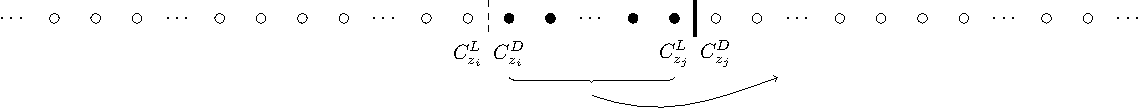
\includegraphics[scale = 0.8]{poglavlja/palindromi/slike/odredjenost-korak1-crop.pdf}
	\end{figure}

	Koristeći komplementarnost elemenata palindroma $z_i$ s
	obzirom na centar palindroma $z_i$ (puna linija)
	poznati elementi jedinstveno određuju nove elemente.

	\begin{figure}[htb!]
	\centering%
	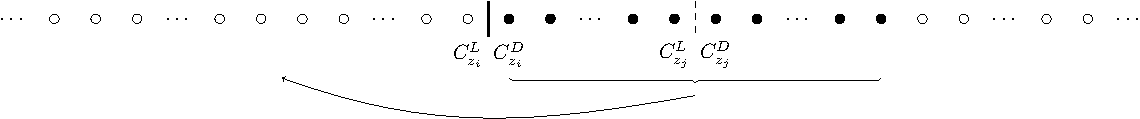
\includegraphics[scale = 0.8]{poglavlja/palindromi/slike/odredjenost-korak2-crop.pdf}
	\end{figure}

	Isti se pristup (naizmjenično korištenje komplementarnosti elemenata palindroma)
	sada primjenjuje sve dok se cijeli palindromi ne ispune.

\end{proof}

\begin{napomena_}
	\label{pal:nap:oblikpresjecenihpalindroma}
	Iz dokaza leme \ref{lem:opresjekupalindroma} slijedi da za dva palindroma
	$z_i$ i $z_j$ koja se sijeku varijable $(X_{i-m+1},\cdots,X_{j})$
	imaju sljedeću strukturu:

\begin{center}
\begin{tabular}{ttttttttttt}
	&
	$\underbrace{\qquad X_{i-m+1} \cdots X_{i-m+r}}_{\lambda \text{ ili } \ol{\lambda}}$
	&
	$\cdots\lambda$
	&
	$\ol{\lambda}$
	&
	$\underbrace{X_{C_{z_i}^{D}} \cdots X_{C_{z_j}^{D}-1}}_{\lambda}$
	&
	$\ol{\lambda}$
	&
	$\lambda \cdots$
	&
	$\underbrace{X_{j-r+1} \cdots X_{j} \qquad}_{\lambda \text{ ili } \ol{\lambda}}$
	

\end{tabular}
\end{center}

	\noindent
	gdje $\lambda$ predstavlja niz elementa $\left[C_{z_i}^{D},C_{z_j}^{D}\right>$,
	a $\ol{\lambda}$ niz $\ol{\left[C_{z_i}^{D},C_{z_j}^{D}\right>}$.
	Broj znakova u $\lambda$ jest $l=j-i$, a $r$ je ostatak pri cjelobrojnom
	dijeljenju $\frac{m}{2} = q \cdot l + r$.
	Rubni elementi sadrže samo one elemente $\lambda$
	ili $\ol{\lambda}$ koji su potrebni da bi se palindromi ispunili
	(duljina palindroma ne mora nužno biti višekratnik broja elemenata  u $\lambda$).
	Također, početak prvog palindroma i kraj drugog palindroma nalaze se
	u različitim nizovima ($\lambda$ ili $\ol{\lambda}$).
\end{napomena_}

\noindent
Neka je funkcija $S: \mathbb{N} \times \mathbb{N} \times
\mathbb{N} \rightarrow \mathbb{N}^{\mathbb{N}_{0}}$
zadana sa
\begin{gather}
	(S(i,j,k))(0) = i \ ,  \nonumber \\
	\label{pal:eqn:definicijaSniza}
	(S(i,j,k))(n) = 2 \left(j + (n-1)k \right) - (S(i,j,k))(n-1) -1 \ .
\end{gather}

\noindent
Ideja u pozadini definicije funkcije $S$ je da se na
elegantan način opiše ponašanje
(oblik) niza $X_n$ iz napomene 
\ref{pal:nap:oblikpresjecenihpalindroma}.



Definirajmo sada funkciju 
$\xi: \mathbb{N} \times \mathbb{N} \times \mathbb{N} \times \mathbb{N}
\rightarrow [0,1]$ kao vjerojatnost
\[
	\xi(i,j,k,w) =
	\vP \left( X_{S\left( i,j,k \right)(0)} = 
	   \ol{\tsvar{X}}_{S\left( i,j,k \right)(1)} =
	   X_{S\left( i,j,k \right)(2)} =
	   \ol{\tsvar{X}}_{S\left( i,j,k \right)(3)} =
	   \ldots =
	   \ol{\tsvar{X}}_{S\left( i,j,k \right)(w)}
	\right)
\]
za $w$ neparan, dok $\xi$ za $w$ paran definiramo kao
\[
	\xi(i,j,k,w) =
	\vP \left( X_{S\left( i,j,k \right)(0)} = 
	   \ol{\tsvar{X}}_{S\left( i,j,k \right)(1)} =
	   X_{S\left( i,j,k \right)(2)} =
	   \ol{\tsvar{X}}_{S\left( i,j,k \right)(3)} =
	   \ldots =
	   X_{S\left( i,j,k \right)(w)}
	\right) \ .
\]

\noindent
Vrijednosti funkcije $\xi$ možemo računati pomoću leme
\ref{pal:lem:mixvarijabli}.

\begin{pro} \label{pal:pro:opcavjerojatnostpresjeka}
	Pretpostavimo da su $\tsvar{X}_n$ nezavisne slučajne varijable
	te neka je $l = j-i$. Označimo s $q$ i $r$ odgovarajuće
	koeficijente kod cjelobrojnog dijeljenja s ostatkom
	$m/2 = q \cdot l + r$. 
	\begin{itemize}
		\item[a)]{
			za $l \geq m$ ($Y_i$ i $Y_j$ se ne sijeku) vrijedi
			\[
				\vP (\tsvar{Y}_i \cdot \tsvar{Y}_j =1 ) =
				\vP (\tsvar{Y}_i=1) \vP (\tsvar{Y}_j=1) \ ,
			\]
		}
		\item[b)]{
			za $\frac{m}{2} \leq l \leq m-1$ vrijedi
			\begin{multline}
				\vP (\tsvar{Y}_i \cdot \tsvar{Y}_j =1 ) = 
				\prod_{v=i-m+1}^{i-l}
				\xi(v, i-\frac{m}{2}+1, l, 2) \cdot \\
				\prod_{v=i-l+1}^{i-\frac{m}{2}}
				\xi(v, i-\frac{m}{2}+1, l, 1) 
				\prod_{v=j-l+1}^{j-\frac{m}{2}}
				\xi(v, j-\frac{m}{2}+1, l, 1) \ ,
			\end{multline}
		}
		\item[c)]{
			za $l < \frac{m}{2}$ i $2r \leq l$ vrijedi
			\begin{multline}
				\vP (\tsvar{Y}_i \cdot \tsvar{Y}_j =1 ) = 
				\prod_{v=i-m+1}^{i-m+r}
				\xi(v, i-m+r+1, l, 2q+1) \cdot \\
				\prod_{v=2r+1}^{l}
				\xi(v, i-m+r+l+1, l, 2q) 
				\prod_{v=l+1}^{r+l}
				\xi(v, i-m+r+l+1, l, 2q+1) \ ,
			\end{multline}
		}
		\item[d)]{
			za $l < \frac{m}{2}$ i $2r > l$ vrijedi
			\begin{multline}
				\vP (\tsvar{Y}_i \cdot \tsvar{Y}_j =1 ) = 
				\prod_{v=i-m+1}^{i-m+l-2r}
				\xi(v, i-m+r+1, l, 2q+2) \cdot \\
				\prod_{v=i-m+l-2r+1}^{i-m+r}
				\xi(v, i-m+r+l+1, l, 2q+1) 
				\prod_{v=l+1}^{r+l}
				\xi(v, i-m+r+l+1, l, 2q+1) \ .
			\end{multline}
		}

	\end{itemize}
\end{pro}

\begin{proof}

	Tvrdnja a) slijedi iz $l>m-1$ zbog nezavisnosti varijabli
	$\{\tsvar{X}_{i-m+1},\ldots,\tsvar{X}_i\}$ i
	$\{\tsvar{X}_{j-m+1},\ldots,\tsvar{X}_j\}$.

	Zbog $\frac{m}{2} \leq l \leq m-1$ niz $(\tsvar{X}_n)$ ima oblik kao na slici
	\ref{pal:fig:l_vecejednako_k}.
	Iz oblika slijedi da niz $A$ (početnih $m-l$ elemenata)
	mora biti komplementaran nizu $\ol{A}$ te isti kao
	i posljednjih $m-l$ elemenata. Nizovi $B$ i $C$
	međusobno su nezavisni te nezavisni o $A$ (odnosno $\ol{A}$).

\begin{figure}[htb!]
\centering%
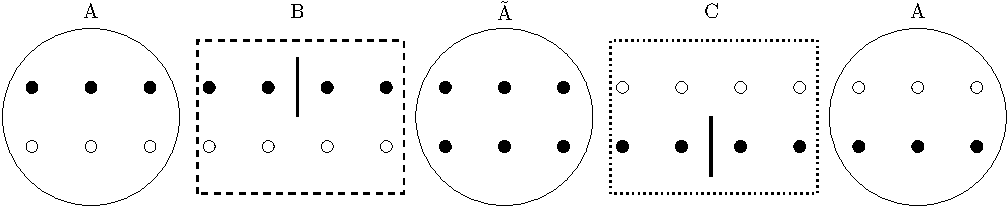
\includegraphics[scale = 0.8]{poglavlja/palindromi/slike/l_vecejednako_k-crop.pdf}
\caption{Primjer povezanosti elemenata dva presijecajuća palindroma (puni krugovi
	predstavljaju elemente palindroma) duljine $m=10$ za $2r \leq l$. Podebljane
	linije između elemenata predstavljaju sredine palindroma.}
\label{pal:fig:l_vecejednako_k}
\end{figure}

	\noindent
	Stoga, koristeći nezavisnost, funkciju $S$ i lemu \ref{pal:lem:mixvarijabli} dobivamo
	tvrdnju b).
%
\begin{multline*}
	\vP (\tsvar{Y}_i \cdot \tsvar{Y}_j =1 ) = 
	\prod_{t=m-1}^{l}
	\underbrace{
		\vP \left(
		\tsvar{X}_{i-t} =
		\ol{X}_{S(i-t, i-\frac{m}{2}+1, l)(1)} = 
		\tsvar{X}_{S(i-t, i-\frac{m}{2}+1, l)(2)} 
		\right)
	}_{\text{odnos A i \~A}}
	\cdot \\
	\prod_{t=k}^{l-1}
	\left[
		\underbrace{
		\vP \left(
		\tsvar{X}_{i-t} =
		\ol{X}_{S(i-t, i-\frac{m}{2}+1, l)(1)}
		\right)
		}_{B}
		\underbrace{
		\vP \left(
		\tsvar{X}_{j-t} =
		\ol{X}_{S(j-t, j-\frac{m}{2}+1, l)(1)}
		\right)
		}_{C}
	\right] = \\
		\prod_{v=i-m+1}^{i-l}
		\xi(v, i-\frac{m}{2}+1, l, 2) 
		\prod_{v=i-l+1}^{i-\frac{m}{2}}
		\xi(v, i-\frac{m}{2}+1, l, 1) 
		\prod_{v=j-l+1}^{j-\frac{m}{2}}
		\xi(v, j-\frac{m}{2}+1, l, 1) 
\end{multline*}

\noindent
	Slika \ref{pal:fig:2r_vece_l} prikazuje
	slučaj $2r>l$ i $l<\frac{m}{2}$. Budući da je $2r>l$ prvih $2r-l$ elemenata
	nalazi se u nizu $2q+3$ puta (uz komplementarnost na odgovarajućim
	mjestima), dok se ostalih $l-r$ elemenata na početku i na kraju
	nalazi u nizu $2q+1$ puta (uz komplementarnost na odgovarajućim
	mjestima).
	Stoga, koristeći nezavisnost, funkciju $S$ i lemu \ref{pal:lem:mixvarijabli} dobivamo
	tvrdnju d).
%
\begin{figure}[htb!]
\centering%
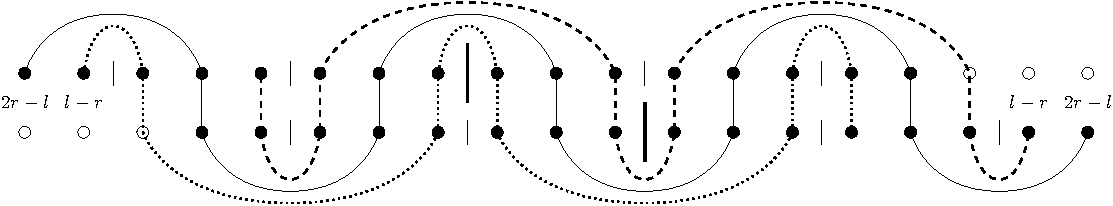
\includegraphics[scale = 0.8]{poglavlja/palindromi/slike/2r_vece_l-crop.pdf}
\caption{Primjer povezanosti elemenata dva presijecajuća palindroma (puni krugovi
	predstavljaju elemente palindroma) duljine $m=16$ za $2r>l$. Podebljane
	linije između elemenata predstavljaju sredine palindroma, a obične linije
	mjesta nužne simetrije.}
\label{pal:fig:2r_vece_l}
\end{figure}


	Ideja dokaza tvrdnje d) može se primjeniti i na tvrdnju c)
	pazeći da sada u početnom i krajnjem dijelu nemamo
	elemente koji se pojavljuju $2q+3$ puta.
\end{proof}

\begin{kor} \label{pal:kor:njdvjerojatnostpresjeka}
	Pretpostavimo da su $\tsvar{X}_n$ nezavisne jednako distribuirane slučajne
	varijable
	te neka je $l = j-i$. Označimo s $q$ i $r$ odgovarajuće
	koeficijente kod cjelobrojnog dijeljenja s ostatkom
	$\frac{m}{2} = q \cdot l + r$. Tada vrijedi
	\begin{itemize}
		\item[a)]{
			\text{za } $\frac{m}{2} \leq l \leq m-1$
			\[
				\vP( \tsvar{Y}_i \cdot \tsvar{Y}_j =1 ) =
				\left(
					\sum_{x \in \mathcal{A}} p_x^2 p_{\ol{x}} 
				\right)^{m-l}
				\left(
					\sum_{x \in \mathcal{A}} p_x p_{\ol{x}} 
				\right)^{2l-m}
			\]
		}
		\item[b)]{
			\text{za } $l < q$ i $2r \leq l$
			\[
				\vP( \tsvar{Y}_i \cdot \tsvar{Y}_j =1 ) =
				\left(
				\sum_{x \in \mathcal{A}} p_x^{q+1} p_{\ol{x}}^{q+1} 
				\right)^{2r}
				\left(
				\sum_{x \in \mathcal{A}} p_x^{q+1} p_{\ol{x}}^{q} 
				\right)^{l-2r}
			\]
		}
		\item[c)]{
			\text{za } $l < q$ i $2r > l$
			\[
				\vP( \tsvar{Y}_i \cdot \tsvar{Y}_j =1 ) =
				\left(
				\sum_{x \in \mathcal{A}} p_x^{q+1} p_{\ol{x}}^{q+1} 
				\right)^{2l-2r}
				\left(
				\sum_{x \in \mathcal{A}} p_x^{q+1} p_{\ol{x}}^{q+2} 
				\right)^{2r-l}
			\]
		}
	\end{itemize}
\end{kor}

\begin{proof}
Iz nezavisnosti i jednake distribuiranosti slučajnih varijabli
$X_n$, napomene \ref{pal:nap:njdmixvarijabli} te propozicije
\ref{pal:pro:opcavjerojatnostpresjeka} slijedi tvrdnja korolara.
\end{proof}

\noindent
Tvrdnju korolara \ref{pal:kor:njdvjerojatnostpresjeka}
kao i dokaz 
može se naći i u radu \textcite{leung_nonrandom_2005}. 

\begin{napomena_} \label{pal:nap:kovarijanca}
Koristeći lemu \ref{pal:lem:meanvarpalindroma} i propoziciju \ref{pal:pro:opcavjerojatnostpresjeka}
(jednakosti \ref{pal:eqn:meanpalindromanjd} i \ref{pal:eqn:varpalindromanjd} te korolar \ref{pal:kor:njdvjerojatnostpresjeka} u
n.j.d. slučaju) kovarijanca $\vCov{Y_i, Y_j}$ može se izračunati budući da vrijedi
\begin{gather}
	\vCov{\tsvar{Y}_i, \tsvar{Y}_j} =
	\vE{\tsvar{Y}_i \cdot \tsvar{Y}_j} - \vE{\tsvar{Y}_i} \vE{\tsvar{Y}_j}
	= \vP \left( \tsvar{Y}_i \cdot \tsvar{Y}_j  =1 \right)
	- \vP \left( \tsvar{Y}_i =1 \right) \vP \left( \tsvar{Y}_j  =1\right)
\end{gather}
\end{napomena_}

\begin{kor}
	Pretpostavimo da su $\tsvar{X}_n$ nezavisne jednako distribuirane slučajne
	varijable s uniformnom distribucijom nad abecedom $\mathcal{A}$.
	Tada su pojavljivanja palindroma na mjestu $i$ i mjestu $j$
	nezavisna za $i \neq j$. Odnosno, vrijedi jednakost
	\[
		\vP( \tsvar{Y}_i \cdot \tsvar{Y}_j =1 ) =  
		\vP( \tsvar{Y}_i=1) \vP( \tsvar{Y}_j=1) \ .
	\]
\end{kor}

\begin{proof}
	Ukoliko se palindromi ne sijeku	nezavisnost je očita.
	Ako se pak sijeku,
	za $\beta=\frac{1}{|\mathcal{A}|}$
	iz korolara \ref{pal:kor:njdvjerojatnostpresjeka} slijedi
	\begin{itemize}
		\item[a)]{
			\text{za } $\frac{m}{2} \leq l \leq m-1$
			\[
				\vP (\tsvar{Y}_i \cdot \tsvar{Y}_j =1 ) =
				\left(
					\sum_{x \in \mathcal{A}} \beta^2 \cdot \beta 
				\right)^{m-l}
				\left(
					\sum_{x \in \mathcal{A}} \beta \cdot \beta 
				\right)^{2l-m}
				=
				\left(
					\beta^2
				\right)^{m-l}
				\left(
					\beta
				\right)^{2l-m}
				=
				\beta^{m} \ ,
			\]
		}
		\item[b)]{
			\text{za } $l < q$ i $2r \leq l$
			\[
				\vP (\tsvar{Y}_i \cdot \tsvar{Y}_j =1 ) =
				\left(
				\sum_{x \in \mathcal{A}} \beta^{q+1} \beta^{q+1} 
				\right)^{2r}
				\left(
				\sum_{x \in \mathcal{A}} \beta^{q+1} \beta^{q} 
				\right)^{l-2r}
				=
				\left(
				\beta^{2q+1} 
				\right)^{2r}
				\left(
				\beta^{2q}
				\right)^{l-2r}
				=
				\beta^{m} \ ,
			\]
		}
		\item[c)]{
			\text{za } $l < q$ i $2r > l$
			\begin{multline*}	
				\vP (\tsvar{Y}_i \cdot \tsvar{Y}_j =1 ) =
				\left(
				\sum_{x \in \mathcal{A}} \beta^{q+1} \beta^{q+1} 
				\right)^{2l-2r}
				\left(
				\sum_{x \in \mathcal{A}} \beta^{q+1} \beta^{q+2} 
				\right)^{2r-l}
				\\
				=
				\left(
				\beta^{2q+1}
				\right)^{2l-2r}
				\left(
				\beta^{2q+2}
				\right)^{2r-l}
				=
				\beta^{m} \ .
			\end{multline*}
		}
	\end{itemize}
	%
	Nezavisnost sada slijedi iz 
	\ref{pal:pro:opcavjerojatnostpresjeka}
	budući da vrijedi
	\[
		\vP( \tsvar{Y}_i = 1) =
		\prod_{j=1}^{\frac{m}{2}} \left[
		\sum_{x \in \mathcal{A}}
		\beta \beta
		\right]
		=
		\beta^{\frac{m}{2}} \ , \quad
		\vP( \tsvar{Y}_i = 1) \vP(\tsvar{Y}_j = 1)
		= \beta^{2 \cdot \frac{m}{2}} = \beta^{m} \ .
	\]
\end{proof}
